\chapter{Introduction}
You should be able to define and understand the following after finishing these notes. 
\begin{itemize}
    \item Complexity theory, universal computation models, universal turing machine, Church-Turing thesis and its other forms, hypercomputation, random algorithm and probabilistic Turing machine, probabilistic Church-Turing thesis, Deutsch notion of universal quantum computiong, discrete logarithm and Shor's algorithm, Grover's algorithm and space searching, error correcting codes, CSS codes, superdense coding, reversing zero channel, RSA and cryptosystems, Diaffie-Hallamn.
    \item Bell-EPR pair and no classical explanation, Maxwell's deamon, Szilards' engine adn exorcism. 
    \item Reversible computation, billiard ball model, Fredkin, Conservative logic
\end{itemize}

Before any formal approach we give a brief introduction to quantum computing concepts and application. We model a \textit{quantum state space} with a vector space (Hilbert space to be exact)\footnote{Non-linear behavior can lead to time-travel, faster than light communication, and violation of second law of thermodynamics}. Each vector represent a \textit{quantum state} and can be thought of a \textit{superposition} of some basis state. A quantum bit or \textit{qubit} is an example of 2-dimensional quantum system with \(\ket{0}\) and \(\ket{1}\) as basis and a state \(\ket{\psi}\) can be represented by 
\begin{equation*}
    \ket{\psi} = \alpha \ket{0} + \beta \ket{1} \quad \alpha, \beta \in \Complex
\end{equation*}
We may also consider a normalization condition for such state. That is, we must have \(\abs{\alpha}^2 + \abs{\beta}^2 = 1\). We can interpret this coefficients to be the probability of result of measuring \(\ket{\psi}\). That is, \(\prob{M \ket{\psi} = \ket{0}} = \abs{\alpha}^2\) and \(\prob{M \ket{psi} = \ket{1}} = \abs{\beta}^2\). Because of the normalization condition, we can write \(\ket{\psi}\) as 
\begin{equation*}
    \ket{\psi} = e^{i\gamma} \bracket{\cos \dfrac{\theta}{2} \ket{0} + \sin \dfrac{\theta}{2} e^{i\phi} \ket{1}}
\end{equation*}
dropping the \(e^{i\gamma}\) factor allows us to represent the state space on a sphere called \textit{Bloch sphere}.
\begin{figure}
    \centering
    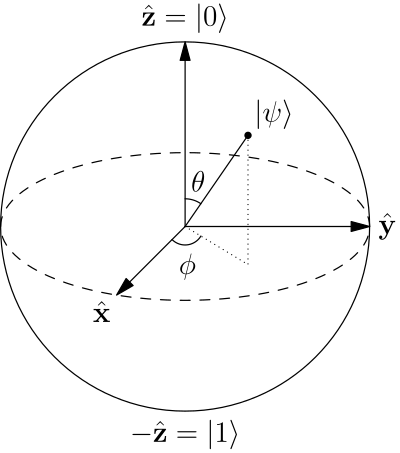
\includegraphics[width = 0.5\textwidth]{Chapters/Graphics/Bloch_Sphere.png}
    \caption{Bloch sphere}
\end{figure}

Suppose we have two qubits then the basis of the system is \(\set{\ket{00}, \ket{01} , \ket{10} , \ket{11}}\) and every state is represent in a superposition of this basis
\begin{equation*}
    \ket{\psi} = \sum_{x \in \set{0,1}^2} \alpha_x \ket{x} \quad \text{with} \quad \sum_{x \in \set{0,1}^2} \abs{\alpha_x}^2 = 1
\end{equation*}
If we measure the first we get \(\ket{0}\) with probability 
\begin{equation*}
    \abs{\alpha_{00}}^2 + \abs{\alpha_{01}}^2 
\end{equation*}
and the post-measurement state would be 
\begin{equation*}
    \ket{\psi'} = \dfrac{\alpha_{00} \ket{00} + \alpha_{01} \ket{01}}{\sqrt{\abs{\alpha_{00}}^2 + \abs{\alpha_{01}}^2}}
\end{equation*}
Bell state or EPR pair is 
\begin{equation*}
    \dfrac{\ket{00} + \ket{11}}{\sqrt{2}}
\end{equation*}
A state of multiple qubit is called \textit{separable} if each of the qubit is in a definite state i.e. we can write it as a tensor product. Otherwise, they are in an \textit{entangled} state.


\section{Quantum gates and measurements}

Isolated quantum mechanic processes (evolution) are represent by unitary matrices \(U U^{\dagger} = I\). Some example of quantum gates include
\begin{align*} 
    \sigma_x &= X = \begin{bmatrix}
        0 & 1 \\
        1 & 0
    \end{bmatrix} \quad \text{Quantum NOT gate}\\
    \sigma_y &= Y = \begin{bmatrix}
        0 & -i \\
        i & 0
    \end{bmatrix} \quad \text{Y gate}\\
    \sigma_z &= Z = \begin{bmatrix}
        1 & 0 \\
        0 & -1
    \end{bmatrix} \quad \text{Z gate}\\
    H &= \dfrac{1}{\sqrt{2}} \begin{bmatrix}
        1 & 1 \\
        1 & -1
    \end{bmatrix} \quad \text{Hadamard gate}\\
\end{align*}
The first three gate correspond to \(180^{\circ}\) rotation along the \(x,y,\) and \(z\) respectively, and are called the \textit{Pauli rotation matrices}. Every gate on a qubit can be viewed as a set of rotations along the \(x,y,z\)-axis of the Bloch sphere. Furthermore, every unitary matrix can be viewed geomtrically as scaling-rotation-scaling. A \textit{Controlled NOT} gate is a two qubit gate 
\begin{figure}
    \centering
    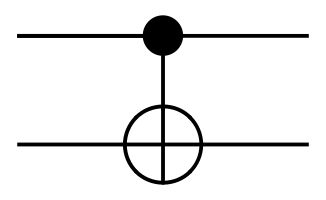
\includegraphics[width = 0.3\textwidth]{Chapters/Graphics/CNOT_Gate.png}
    \caption{CNOT gate}
\end{figure}
that given \(\ket{\psi} \) and \(\ket{\phi}\) input, gives \(\ket{\psi}\) and \(\ket{\psi \oplus \phi}\). The matrix of CNOT gate is 
\begin{equation*}
    U_{CNOT}  = \begin{bmatrix}
        1 & 0 & 0 & 0 \\
        0 & 1 & 0 & 0 \\
        0 & 0 & 0 & 1 \\
        0 & 0 & 1 & 0 \\
    \end{bmatrix}
\end{equation*}

Quantum gates need to be reversible, that is given the output one can find out the output. For example, classical NOT gate is reversible and XOR gate is non-reversible. All multiple qubit gate may be decomposed to CNOT and other single qubit gates. Feedback, FANIN (irreversible) , FANOUT (cloning) are not allowed in quantum computing. In general, Controlled-\(U\) gate is shown as
\begin{figure}
    \centering
    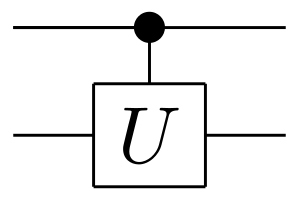
\includegraphics[width = 0.3\textwidth]{Chapters/Graphics/Controlled_Gate.png}
    \caption{Controlled-\(U\) gate}
\end{figure}
and has matrix representation
\begin{equation*}
    \text{Controlled} U = \begin{bmatrix}
        I_n & 0 \\
        0 & U \\
    \end{bmatrix}
\end{equation*}
and measurement of a quantum state is represent by 
\begin{figure}
    \centering
    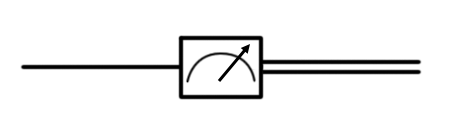
\includegraphics[width = 0.3\textwidth]{Chapters/Graphics/Measurement.png}
    \caption{Measurement}
\end{figure}

No cloning theorem states that lossless copying of qubit using unitary devices can obly be done on orthogonal basis. That is, if \(\ket{\psi}\) can be copied to \(\ket{\phi}\) then 
\begin{equation*}
    \braket{\phi}{\psi} = \begin{cases}
        0 & \psi \perp \phi\\
        1 & \psi = \phi
    \end{cases}
\end{equation*}


\section{Quantum teleportation}
The other Bell states are 
\begin{align*}
    \ket{\beta_{00}} &= \dfrac{\ket{00} + \ket{11}}{\sqrt{2}}\\
    \ket{\beta_{01}} &= \dfrac{\ket{01} + \ket{10}}{\sqrt{2}}\\
    \ket{\beta_{10}} &= \dfrac{\ket{00} - \ket{11}}{\sqrt{2}}\\
    \ket{\beta_{11}} &= \dfrac{\ket{01} - \ket{10}}{\sqrt{2}}
\end{align*}
which are generated by the following circuit --insert diagram Hadamard on the frist qubit and CNOT on the second 
with matrix 
\begin{equation*}
    U = \begin{bmatrix}
        \frac{1}{\sqrt{2}} & 0 & \frac{1}{\sqrt{2}} & 0\\
        0 & \frac{1}{\sqrt{2}} & 0 & \frac{1}{\sqrt{2}} \\
        0 & \frac{1}{\sqrt{2}} & 0 & -\frac{1}{\sqrt{2}} \\
        \frac{1}{\sqrt{2}} & 0 & - \frac{1}{\sqrt{2}} & 0
    \end{bmatrix} = \begin{bmatrix}
        \ket{\beta_{00}} & \ket{\beta_{01}} & \ket{\beta_{10}} & \ket{\beta_{11}}
    \end{bmatrix}
\end{equation*}
Suppose Alice and Bob have an EPR pair \(\ket{\beta_{00}}\), and each took one the pairs. Alice then wants to communicate to Bob the state \(\ket{\psi}\) using only classical bit. Alice and Bob can implement the following -- insert diagram CNOT on Alice qubit, Hadamard on psi, measure psi and alice qubit, not gate on bob and measured alice and Z gate on bob and measure psi. 
\begin{align*}
    \ket{\psi_0} &= \dfrac{\alpha \ket{0} \bracket{\ket{00} + \ket{11}} +  \beta \ket{1} \bracket{\ket{00} + \ket{11}}}{\sqrt{2}}\\
    \ket{\psi_1} &= \dfrac{\alpha \ket{0} \bracket{\ket{00} + \ket{11}} +  \beta \ket{1} \bracket{\ket{10} + \ket{01}}}{\sqrt{2}}\\
    \ket{\psi_2} &= \dfrac{\alpha \ket{+} \bracket{\ket{00} + \ket{11}} +  \beta \ket{-} \bracket{\ket{00} + \ket{11}}}{\sqrt{2}}\\
    &=  \dfrac{1}{2} \ket{00} \bracket{\alpha \ket{0} + \beta \ket{1}} + \dfrac{1}{2} \ket{01} \bracket{\beta \ket{0} + \alpha \ket{1}} \\ \quad &+ \dfrac{1}{2} \ket{10} \bracket{\alpha \ket{0} - \beta \ket{1}} + \dfrac{1}{2} \ket{11} \bracket{\beta \ket{0} - \alpha \ket{1}}\\
    &= \dfrac{1}{2} \ket{00}  \ket{\psi} + \dfrac{1}{2} \ket{01}  \ket{X\psi} + \dfrac{1}{2} \ket{10}  \ket{Z\psi} + \dfrac{1}{2} \ket{11}  \ket{XZ\psi}
\end{align*}
Therefore, after measurements and applying X and Z gates, Bob will have \(\ket{\psi}\). Quantum teleportation is related to quantum erroc correcting codes.

\section{Reversible computing}
A Turing machine \(\calM\) is said to be reversible if there exists another Turing machine \(\calM'\) such that for every configuration change \(c \to c'\) in \(\calM\), there is the configuration change \(c' \to c\) in \(\calM'\).

\begin{theorem}[Bennett 1973]
    For every function \(f\) computable by a one-tape Turing machine in time \(\func{t}{n}\), there is a three-tape reversible Turing machine computing the following mapping within a constant time overhead.
    \begin{equation*}
        a \mapsto (a,\func{j}{a}, \func{f}{a})
    \end{equation*}
    where \(\func{j}{a}\) is ``garbage''. To remove the garbage
    \begin{description}
        \item [Compute \(f\):] \(a \mapsto (a,\func{j}{a}, \func{f}{a})\).
        \item [Fanout: ]\( (a,\func{j}{a}, \func{f}{a}) \mapsto (a,\func{j}{a}, \func{f}{a},\func{f}{a})\).
        \item [Uncompute \(f\):] \( ( (a,\func{j}{a}, \func{f}{a},\func{f}{a}) \mapsto (a,\func{f}{a})\).
    \end{description}
\end{theorem}

Can Quantum computer simulat classical circuits? Yes; since any classical circuit can be replaced by reversible elements such as Toffoli gate (--insert diagram for Toffoli gate, NAND , and FANOUT). The matrix representation of Toffoli gate 
\begin{equation*}
    U = \begin{bmatrix}
        1 & 0 & 0 & 0 & 0 & 0 &0 & 0\\
        0 & 1 & 0 & 0 & 0 & 0 &0 & 0\\
        0 & 0 & 1 & 0 & 0 & 0 &0 & 0\\
        0 & 0 & 0 & 1 & 0 & 0 &0 & 0\\
        0 & 0 & 0 & 0 & 1 & 0 &0 & 0\\
        0 & 0 & 0 & 0 & 0 & 1 &0 & 0\\
        0 & 0 & 0 & 0 & 0 & 0 &0 & 1\\
        1 & 0 & 0 & 0 & 0 & 0 &1 & 0\\
    \end{bmatrix}
    = \begin{bmatrix}
        I_6 & 0 \\
        0 & X\\
    \end{bmatrix}
\end{equation*}
Note that FANOUT creates entangled copies of the quantum state hence it does not violate the no cloning theorems.
We can even assume that classical computer can make random bit. It is easy to see that by using Hadamard gate and then measuring it, quantum computers can make random bits. --insert diagram

\section{Quantum Algorithms and parallelism}
Let \(f : \set{0,1} \to \set{0,1}\) and \(U_f\) be \(\ket{x,y} \mapsto \ket{x, \func{f}{x} \oplus y}\).
\begin{equation*}
    U_f = \begin{bmatrix}
        \func{f'}{0} & \func{f}{0} & 0 & 0\\
        \func{f}{0} & \func{f'}{0} & 0 & 0\\
        0 & 0 & \func{f'}{1} & \func{f}{1}\\
        0 & 0 \func{f}{1} & \func{f'}{1} 
    \end{bmatrix}
\end{equation*}
--insert diagram of Uf and Hadamard
Applying \(\ket{+,0}\) to \(U_f\) gives 
\begin{align*}
    U_f \ket{+,0} &= \dfrac{1}{\sqrt{2}} U_f \ket{00} +  \dfrac{1}{\sqrt{2}} U_f \ket{10}\\
    &= \dfrac{1}{\sqrt{2}} \bracket{\func{f'}{0}\ket{00} + \func{f}{0}\ket{01}} + \dfrac{1}{\sqrt{2}} \bracket{\func{f'}{1}\ket{10} + \func{f}{1}\ket{11}}\\
    &= \dfrac{\ket{0,\func{f}{0}} + \ket{1,\func{f}{1}}}{\sqrt{2}}
\end{align*}
Hence, with a single operation we can "evaluate" \(f\) for all values. Using Hadamard-Welsh Transform we can do this for any function.
\subsection{Deutsch Algorithm}

Let \(f : \set{0,1}^n \to \set{0,1}\) with \(U_f\). Similar to parallelism is one-bit case we can have 
\begin{equation*}
    U_f \ket{0\dots0 , 0} = \dfrac{1}{\sqrt{2^n}} \sum_{x \in \set{0,1}^n} \ket{x} \otimes \ket{\func{f}{x}}
\end{equation*}
using inference property/ measure (will be like the classical case) we can extract information about \(f\). For example, in Deutsch algorithm we use \(U_f\) and construct the following --insert diagram 
\begin{align*}
    \ket{\psi_0} &= \ket{01} \\
    \ket{\psi_1} &= \dfrac{1}{2} \bracket{\ket{00} + \ket{01} + \ket{10}+ \ket{11}}\\
    \ket{\psi_2} &= U_f \ket{\psi_1} \\
    &= \dfrac{1}{2} \begin{bmatrix}
        \func{f'}{0} - \func{f}{0}\\
        \func{f}{0} - \func{f'}{0}\\
        \func{f'}{1} - \func{f}{1}\\
        \func{f}{1} - \func{f'}{1}
    \end{bmatrix}
    \intertext{let \(p_0 = \func{f'}{0} - \func{f}{0}\) and \(p_1 \func{f'}{1} - \func{f}{1}\) then}
    &= \dfrac{1}{2} \bracket{p_0 \ket{00} - p_0 \ket{01} + p_1 \ket{10} - p_1 \ket{11}}\\
    &= \dfrac{1}{2} \bracket{p_0 \ket{0} + p_1 \ket{1}} \otimes \bracket{\ket{0} - \ket{1}} \\
    &= \begin{cases}
        (-1)^{\func{f}{0}} \ket{+} \otimes \ket{-} & \func{f}{0} = \func{f}{1} \\
        (-1)^{\func{f}{0}} \ket{-} \otimes \ket{-} & \func{f}{0} \neq \func{f}{1} 
    \end{cases}\\
    \ket{\psi_3} &= \begin{cases}
        (-1)^{\func{f}{0}} \ket{0} \otimes \ket{-} & \func{f}{0} = \func{f}{1} \\
        (-1)^{\func{f}{0}} \ket{1} \otimes \ket{-} & \func{f}{0} \neq \func{f}{1} 
    \end{cases}\\
    &= (-1)^{\func{f}{0}} \ket{\func{f}{0} \oplus \func{f}{1}} \otimes \ket{-} 
\end{align*}
hence in one operation we can learn a global property of the function namely the value of \(\func{f}{0} \oplus \func{f}{1}\). A generalization of Deutsch algorithm is the Deutsch-Jozsa algorithm which extends \(f : \set{0,1}^n \to \set{0,1}\). First, consider the \(n\)-qubit Hadamard gate is defined as 
\begin{align*}
    H^{\otimes n} \ket{x_1, \dots, x_n} &= H \ket{x_1} \otimes \dots \otimes H \ket{x_n}\\
    &= \dfrac{1}{\sqrt{2^n}} \sum_{z \in \set{0,1}^n} (-1)^{x \cdot z} \ket{z}
\end{align*}
where \(x \cdot z = x_1z_1 + x_2 z_2 + \dots + x_n z_n\). In particular 
\begin{align*}
    H^{\otimes n} \ket{0 \dots 0} &= \dfrac{1}{\sqrt{2^n}} \bracket{ \ket{0}  + \ket{1}} \otimes \dots \otimes \bracket{\ket{0} + \ket{1}}\\
    &= \dfrac{1}{\sqrt{2^n}} \sum_{x \in \set{0,1}^n} \ket{x}\\
\end{align*}
The Deutsch-Jozsa algorithm works as follow --insert diagram 
\begin{align*}
    \ket{\psi_0} &= \ket{0\dots 0, 1}\\
    \ket{\psi_1} &= \ket{+ \dots +, -} = \dfrac{1}{\sqrt{2^n}} \bracket{\sum_{x \in \set{0,1}^n} \ket{x} } \otimes \ket{-}\\ 
    \ket{\psi_2} &= \dfrac{1}{\sqrt{2^n}} \bracket{\sum_{x \in \set{0,1}^n} (-1)^{\func{f}{x}}\ket{x} } \otimes \ket{-}\\
    \ket{\psi_3} &= \dfrac{1}{2^n} \bracket{\sum_{z \in \set{0,1}^n} \sum_{x \in \set{0,1}^n}  (-1)^{\func{f}{x} + x \cdot z} \ket{z}} \otimes \ket{-}
\end{align*}
Now we can determine whether \(f\) is constant or balance (has the same number of one and zeros) by measuring the first qubit. 
\begin{itemize}
    \item If \(f\) is constant then the amplitude of the first bit is \(1\).
    \item If \(f\) is balanced then the amplitude of the first bit is \(0\).
\end{itemize}
Hence after measuring if \(\ket{0}\) then \(f\) is constant, otherwise \(f\) is balanced. 


\subsection{Quantum algorithms on Fourier}
such as Deutsch-Jozsa and Shor's algorithms. The Fourier transform
\begin{equation*}
    \ket{j} \mapsto \dfrac{1}{\sqrt{2^n}} \sum_{k = 0}^{2^n - 1} e^{2\pi i \frac{jk}{2^n}} \ket{k}
\end{equation*}
is a unitary operation. Fast Fourier transform on classical is \(\bigO{N \lg N}\) and on quantum is \(\bigO{\lg^2 N}\). The quantum Fourier transform and Shor's algorithm can be used to solve a class of problems, the \textit{hidden subgroup problem}. Suppose \(f: G \to X\), where \(G\) is a finitely generated group and \(X\) is a finite set, is such that \(f\) is constant and distinct on the cosets of subgroup \(K\). Given a quantum black box for performing the unitary transformation \(U \ket{g} \ket{h} = \ket{g} \ket{h \oplus \func{f}{g}}\) for \(g \in G\), \(h \in X\), and \(\oplus\) is an appropriately chose binary operation on \(X\), find a generating set for \(K\).

\subsection{Quantum search algorithms}
Such as Grover's algorithm.
Given a set \(S\) of \(N\) points and a property \(P\), find \(n \in S\) such that \(\func{p}{n}\). On classical it can be done in \(\bigO{N}\) but quantum search algorithms are able to do it in \(\bigO{\sqrt{N}}\), a quadratic speed up.
\subsection{Quantum simulation}
\(c^n\) on classical but \(cn\) on quantum, however there is hidden information.
\section{Stern-Gerlach experiment}
Quantum tomography, determining the quantum state of a system.
At small scaled optical techniques have been used to certain degree of success. ion-trap, neutral atom trap, quantum jump, nuclear magnetic resonance (NMR).

\section{Quantum information theory}
\begin{enumerate}
    \item Identify elementary classes of static resources in quantum mechanic, e.g. qubit.
    \item Identify elementary classes of dynamic processes in quantum mechanic, e.g. memory
    \item Quantify resource trade-offs in \(\ast\) current performan dynamic processes.
\end{enumerate}
\subsection{Shannon's noisy/noiseless channel coding theorem}
\begin{itemize}
    \item HSW (Holeve, Shunmacher, Westareland) theorem
    \item Shunmacher's noiseless channel coding theorem
    \item von Neumann entropy agrees with Shannon's entropy if the states are orthogonal. Strictly smaller because of redundancy in non-orthogonal states.
\end{itemize}


Cryptography : Kah96, MooV96, Sch 96a, DL 98 
teleporation and NMR: BBC+93, BBM+ 98, BPM+ 97 , FSB+ 98, NKL 98